% ______________________________________________________________________________
%
%   2DV603 Software Engineering
%   Assignment 1 --- Requirements Engineering
%
%   Author:  Jonas Sjöberg
%            Linnaeus University
%            js224eh@student.lnu.se
%            github.com/jonasjberg
%            www.jonasjberg.com
%
%  License:  Creative Commons Attribution 4.0 International (CC BY 4.0)
%            <http://creativecommons.org/licenses/by/4.0/legalcode>
%            See LICENSE.md for additional licensing information.
% ______________________________________________________________________________


\section{Domain Analysis Document}
Task description from the assignment instructions
\cite{2dv603:assignment1-instructions}:

\begin{quote}
  Perform a domain analysis about ``hotel reservations''. This will help you to
  resolve certain ambiguities that might be present in the above statement of
  requirements.
\end{quote}

\paragraph{Our Goal}
is to create a system to manage front-desk activities at the ``Linnaeus Hotel''.


\subsection{Existing Front-desk Systems}
A very brief look into prior work led to this \cite{2dv603:assignment1-sirvoy}
example of a hotel management system that seemingly includes most features that
are arguably required in order to meet the requirements in this assignment.

A partial screenshot is shown in Figure~\ref{fig:sirvoy}.

Features are grouped by into these main groups:

\begin{itemize}
  \item Booking Engine
  \item Rooms and Rats
  \item Booking Channels (OTAs)
  \item Guest Communication
  \item Booking Management
  \item Service and Support
  \item Payment Processing and Invoicing
\end{itemize}

It is obvious that most of these features stem from the basic features we
likely need to implement in our management system.
Their system has probably grown from a set of basic requirements and use cases,
developing and adding new features over time after customer feedback and
accumulation of domain-specific knowledge and experience.

I find that the functionality for exporting various data to PDF documents,
display in a web front end, e-mailing to customer, etc. are typical examples of
components that can be easily added when the underlying software architecture
is sound.

Another key point is that the domain-specific functionality will not likely
change all too much, and the malleable parts should be made user-adjustable to
fit individual user requirements.

Initial development likely deals mostly with core functionality like domain
logic and transforming pure data. And as development goes on, the core will
likely not see too many invasive changes (assuming a ``good'', flexible design)
and the development effort moves to different means of user interaction, such
as data exporting.

\begin{figure}[htbp]
  \centering
  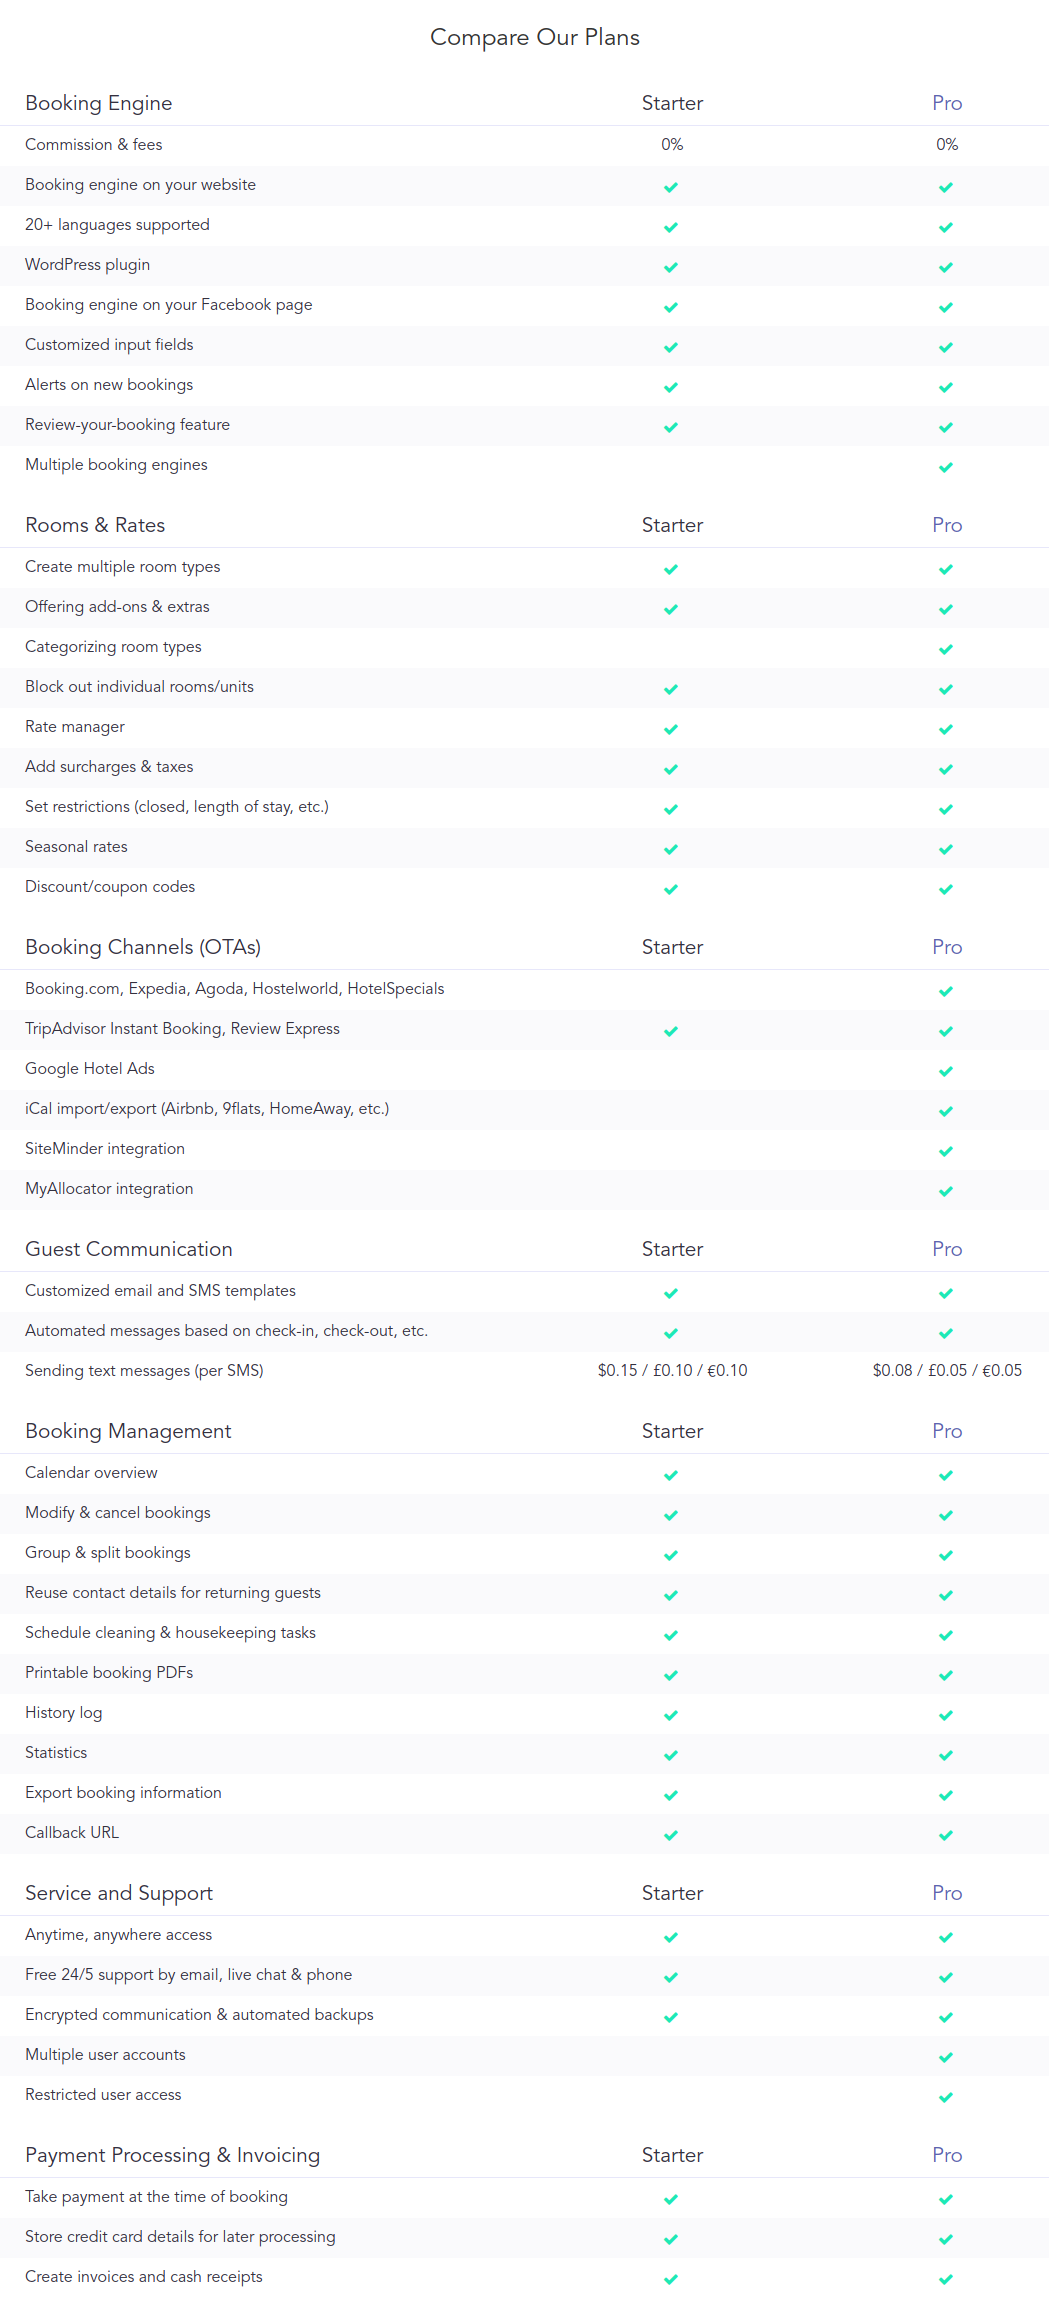
\includegraphics[width=0.7\linewidth]{include/sirvoy.png}
  \caption{Cropped screenshot of features provided by a hotel reservation management system\cite{2dv603:assignment1-sirvoy}}
  \label{fig:sirvoy}
\end{figure}



\subsection{Hotel Reservations Domain Analysis}
%
% TODO: Perform domain analysis about "hotel reservations"..
% This will help resolve certain ambiguities in the requirements statement.
%

\subsubsection{Initial Observations}
Initial assumptions about the domain are based on the description and
information given in the assignment instructions.


Apparent main uses of the system:

\begin{enumerate}
  \item Add, retrieve, modify room reservations
  \item Add, retrieve, modify guest information
  \item ``Real-time'' information provider when staff interact with guests
\end{enumerate}



Characteristics of Hotel Rooms:

\begin{enumerate}
\item Uniquely identified by the room number
\item Smoking/non-smoking
\item Some adjoin other with internal doors between them
\item ``Attractiveness'' (room with a view, room size, etc.) is summarized with a quality level 
\item Contains a fixed number of beds with specific sizes
\item Priced based on quality level (attractiveness)
  \item each quality level has a max daily rate
  \item guests can be up to the max amount
\end{enumerate}

Reservations:

* Deals with specific rooms (availability, requirements)


Data Storage:

* record basic information about each guest, 
    * name, address, telephone number, credit card, passport number


Scenario:

* guest wishes to make a reservation:

  clerk asks about:
      * stay which nights?
      * which type of room do they want?

  System must:

    * verify if room(s) are available on those nights before allowing a reservation to be made
    * verification procedure must take less than 2 seconds to complete.
    * allow requests for specific rooms, controlled by the manage

* overall guests

  system must:
    * record basic information about each guest, 
        * name, address, telephone number, credit card, passport number
    * keep track of the guests account
    * print guests bill.

* guest wishes to cancel a reservation:

    * reservation can be canceled at any time but a percentage of the room
      price may be charged if the cancelation is done too late

* guest checks in

    * room is allocated until checkout
    * must take in average less than 60 seconds to complete

Also, we might assume that the very central core of the system will not be very
complicated. It is purely data storage, retrieval and update (``CRUD'').

Programming is transforming data. This domain will likely not require all too
specific means of transforming data.
Even so, compared to say an online library that might require knownledge of
standards for identification such as ISBN-numbers, DOIs, etc. Most such systems
I've looked at have utilized some sort of automated metadata extraction system,
text search, metadata normalization, comparison, etc. All very difficult
problems that require very advanced techniques.

I would argue that this domain might not be ``computationally'' difficult to
deal with. High risk tasks such as secure payment systems, conformant storage
of user information, etc., can is best solved by integrating third-party
software.

My theory is that the most difficult part of working in this domain is the
human-interaction and usability --- hotel personnel will spend countless hours
with the software and will definitely have a lot of ideas on how it could be
improved to streamline their workflow.

However, we must be provided with this information and \emph{understand it very
well}, as to facilitate us to translate a personal, subjective account of
practical user interaction to requirements/features and finally code.




% System will be used for:
% 
% * Enter reservations
% * Check guests in and out
% 
% Hotel rooms:
% 
% * Room number identifier 
% * Smoking/non-smoking
% * Some adjoin other (internal door between them)
% * Assigned a quality level (room with a view, room size, etc.)
% * Number and types of beds
% * Price depend on quality level
%     * each quality level has a max daily rate
%     * guests can be up to the max amount
% 
% Reservations:
% 
% * Deals with specific rooms (availability, requirements)
% 
% 
% Data Storage:
% 
% * record basic information about each guest, 
%     * name, address, telephone number, credit card, passport number
% 
% 
% Scenario:
% 
% * guest wishes to make a reservation:
% 
%   clerk asks about:
%       * stay which nights?
%       * which type of room do they want?
% 
%   System must:
% 
%     * verify if room(s) are available on those nights before allowing a reservation to be made
%     * verification procedure must take less than 2 seconds to complete.
%     * allow requests for specific rooms, controlled by the manage
% 
% * overall guests
% 
%   system must:
%     * record basic information about each guest, 
%         * name, address, telephone number, credit card, passport number
%     * keep track of the guests account
%     * print guests bill.
% 
% * guest wishes to cancel a reservation:
% 
%     * reservation can be canceled at any time but a percentage of the room
%       price may be charged if the cancelation is done too late
% 
% * guest checks in
% 
%     * room is allocated until checkout
%     * must take in average less than 60 seconds to complete
